\chapter{Stereo Camera Depth Node Implementation}
\label{chapter:stereo_camera_depth}

\section{Theoretical Analysis}\label{subsec:theoretical_analysis}

The obvious drawback of a stereo camera when it comes to depth perception is its limited baseline. It only perceives depth accurately for objects within a certain proximity to the lens. 

Even assuming a perfectly calibrated and rectified camera, the depth estimation is always inaccurate because of disparity errors.

The formula to derive a depth value from a calculated disparity is:

\begin{equation}\label{eq:depth_from_disp}
    z = \frac{f \cdot b}{d}
\end{equation}

Where b is the z is the depth estimate, b is the baseline, f is the focal length, and d is the disparity value.

Taking the derivative of z w.r.t. d, we get

\begin{equation}
    \frac{\partial z}{\partial d} = - \frac{f  \cdot b}{z^2}
\end{equation}

And substituting (\cref{eq:depth_from_disp}) we get:

\begin{equation}
    {\partial z} = \frac{z^2}{f  \cdot b}\partial d
\end{equation}

Where the sign was left away, as for our application, there lies equal danger in a point being perceived as too close and too far away.

For the maximum altitude given a maximum allowable depth error, this yields:

\begin{equation}\label{eq:depth_error_formula}
    z_{\text{max}} = \sqrt{\frac{\Delta z_{\text{max}} \cdot b \cdot f}{\Delta d}}
\end{equation}

$\Delta z$ is the depth error and $\Delta d$ is the disparity error.

The simulated stereo camera in Gazebo had a focal length of 275.42 pixels, and according to the physical stereo camera used on the drone at JPL, a baseline of 0.092 m was used.

With these properties and estimating a subpixel-precision disparity error of 0.5 pixels, the depth error at varying altitudes looks as follows:

\begin{figure}
    \centering
    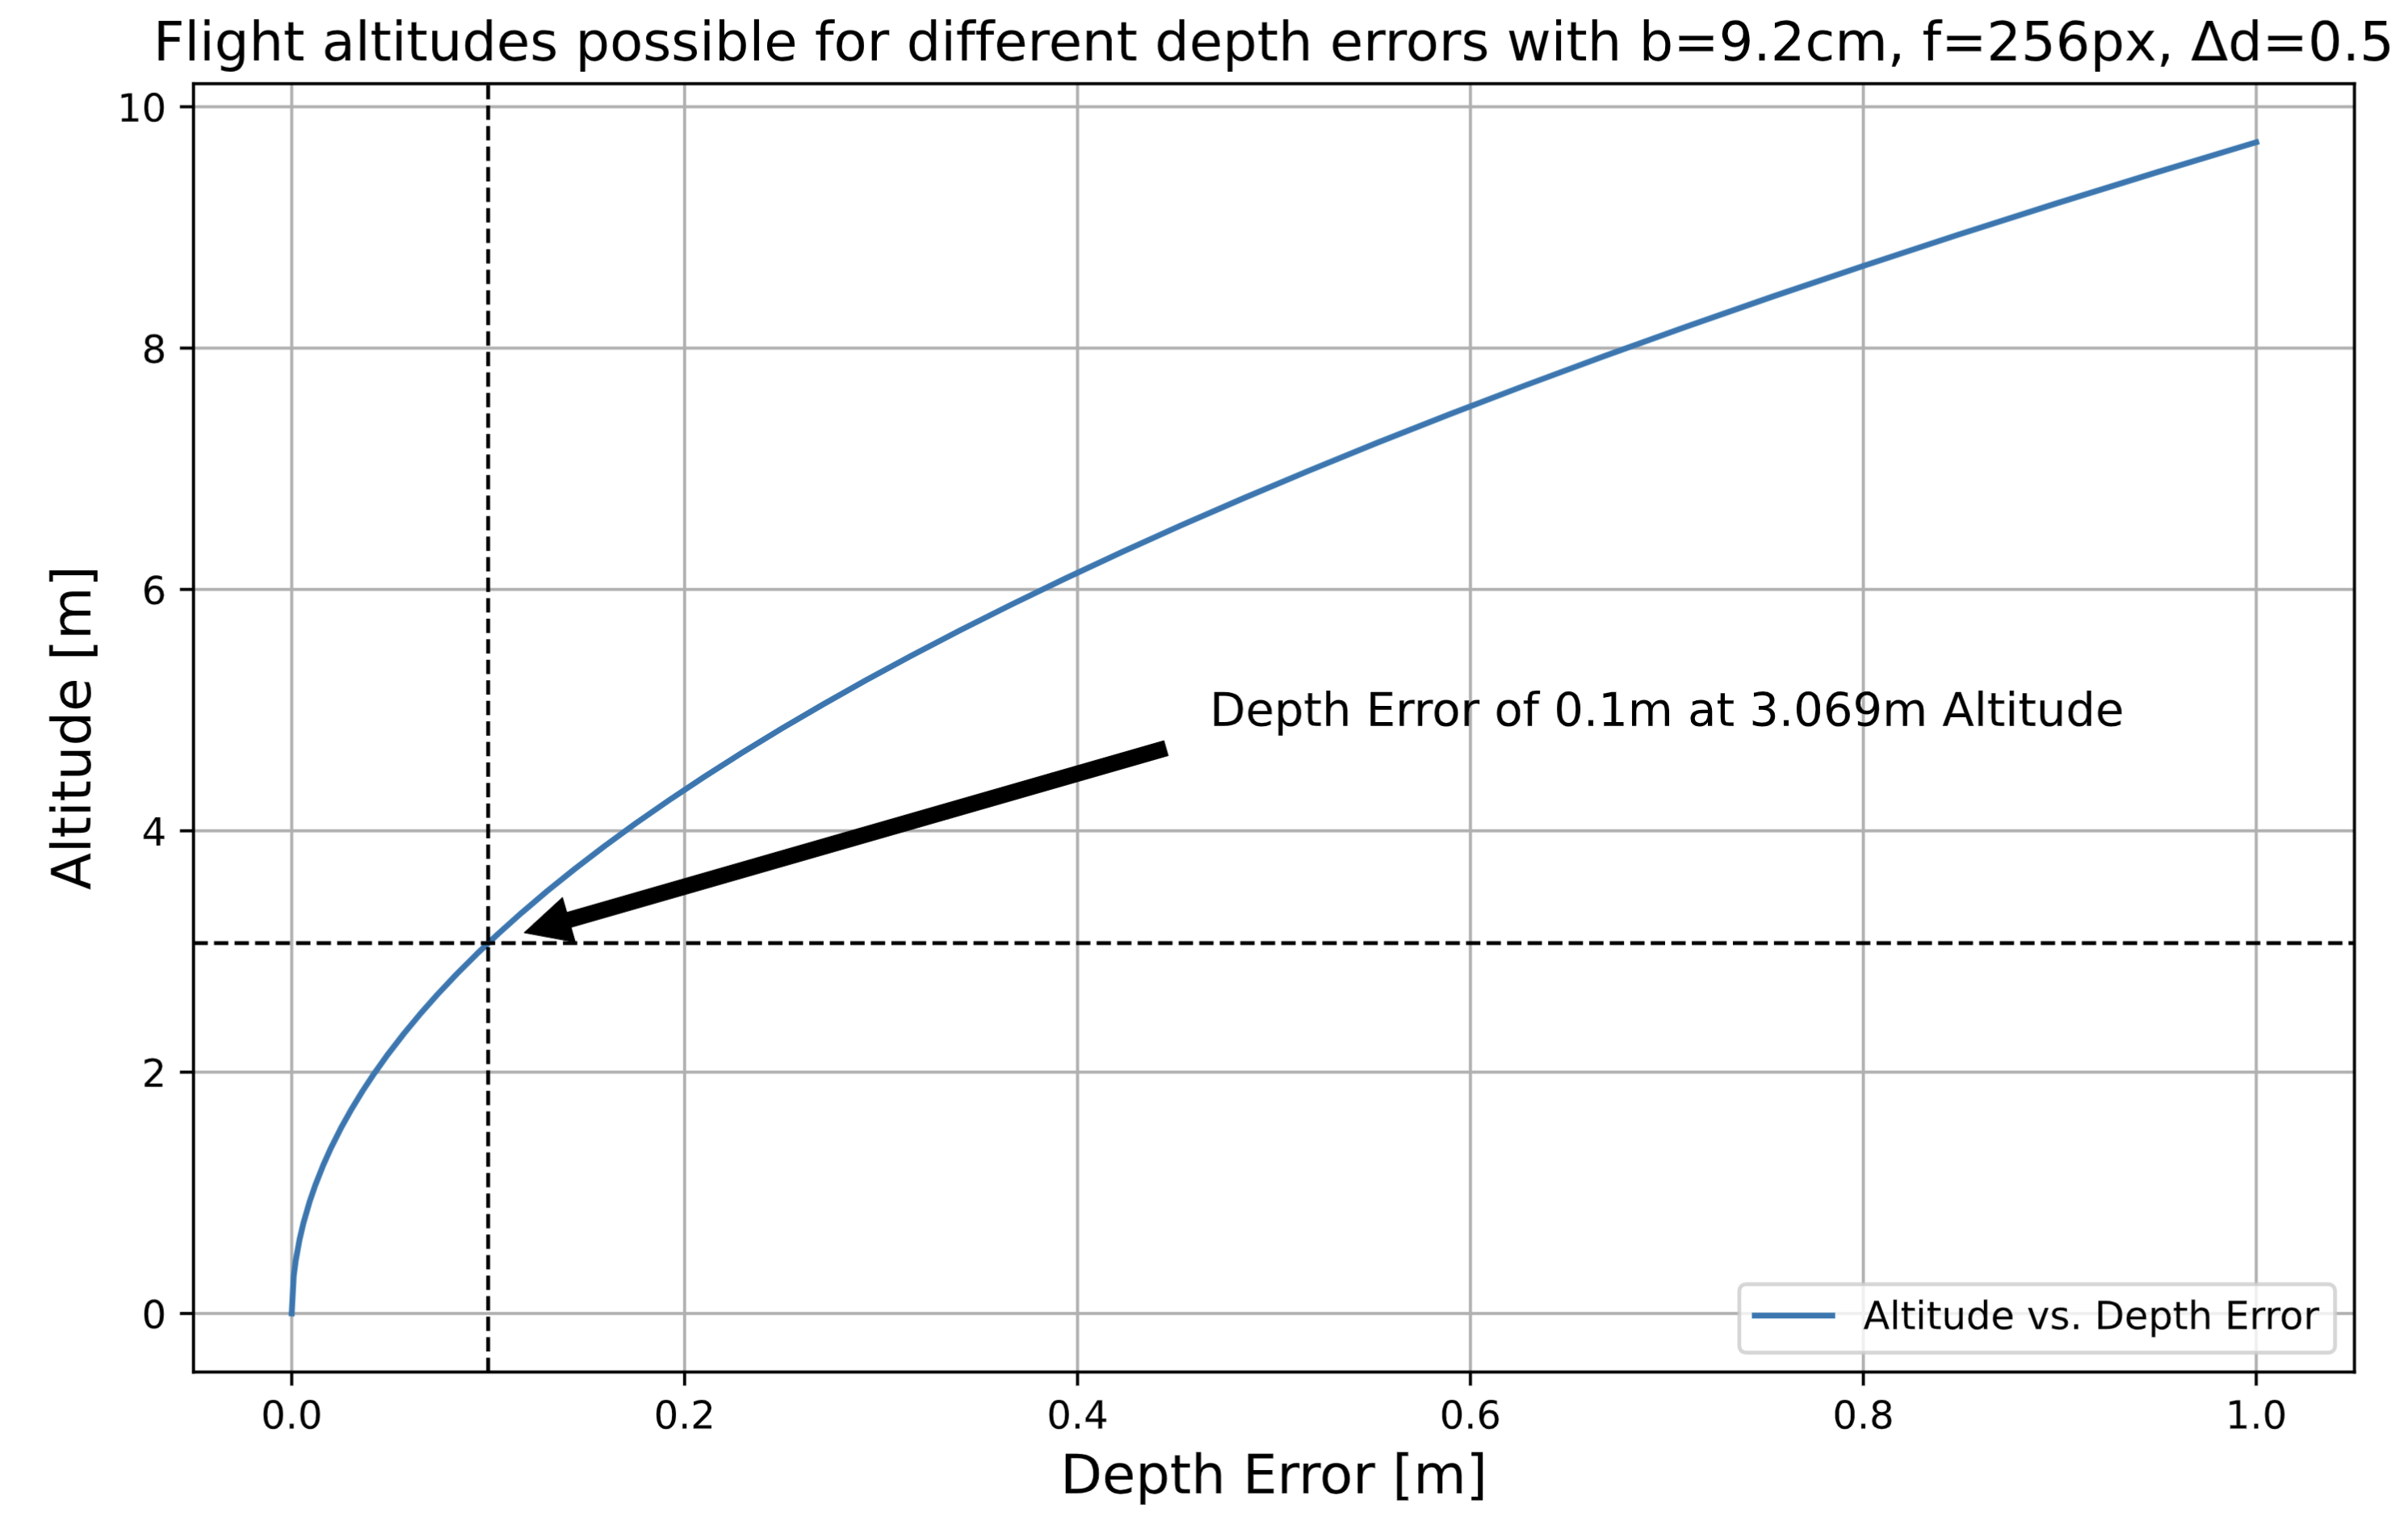
\includegraphics[scale=0.32]{images/stereo_camera_depth/stereo_limit.png}
    \label{fig:stereo_limit}
\end{figure}

Let's assume we allow a maximum depth error of 10 cm. Considering this constraint, we can fly at a maximum altitude of 3.184 m as indicated in \cref{fig:stereo_limit}.

This limitation must be considered. However, it is neither too surprising nor restrictive, as the stereo camera is simply a depth alternative for low-altitude flight maneuvers. In the context of an entire science mission, it is almost exclusively used for landing site verification purposes.

\section{Implementation}

Like Structure from Motion, the stereo depth instance is a ROS node supplied with images and image poses from the xVIO state estimator. As the state estimator was in its final development stages during my thesis, camera images and a ground truth camera pose from the simulation were used instead as input for the stereo algorithm. Note that only one camera pose is given as the second one is derived in a straightforward manner, given the fixed hardware baseline.

\subsection{Stereo Setup Overview}

\cref{fig:drone_sim_setup} shows the drone setup in the simulation with the stereo camera. The stereo camera pair is indicated with the opaque boxes. The large distance to the drone's core is necessary to avoid capturing the landing feet in the image due to the simulation model's discrepancy with the physical drone. As presented in \cref{ch:drone} the drone hardware has landing skids that are spread significantly farther apart than for the simulated model. That is why, when using the stereo camera mounted at the core of the physical drone, the mainstays are not visible in the images detected. In the simulation, they would be detected unless the stereo cameras were positioned further from the rotorcraft's center as shown in \cref{fig:drone_sim_setup}. 

\clearpage %HERE

\begin{figure}
    \centering
    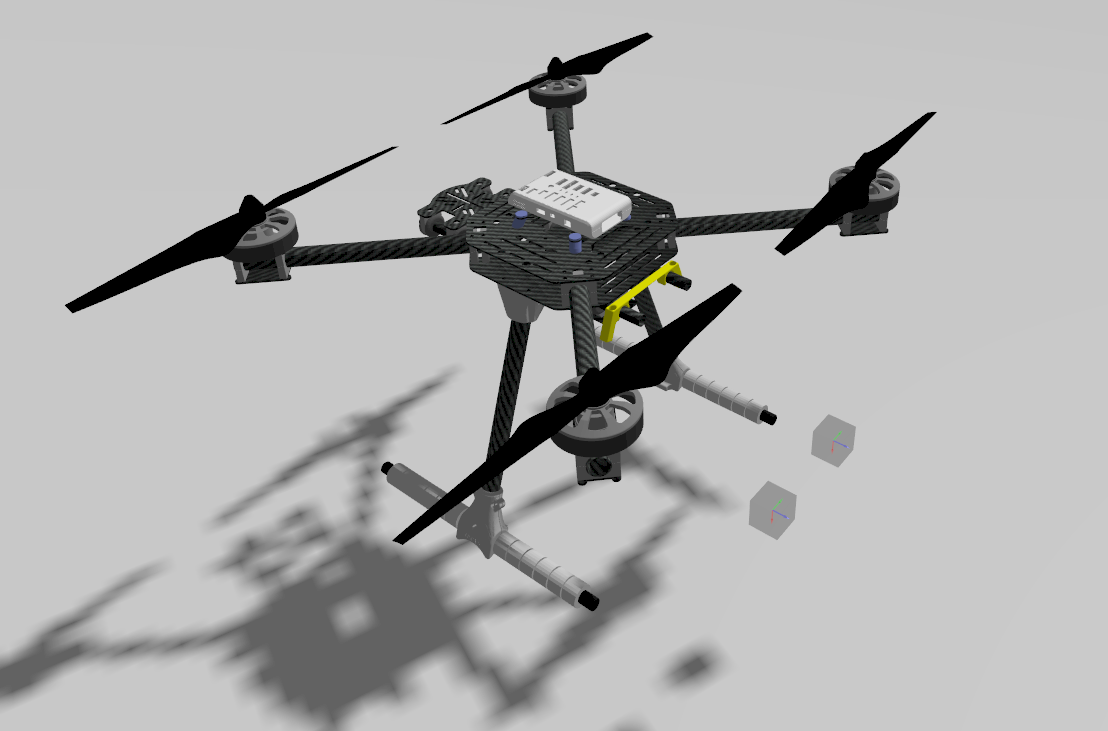
\includegraphics[scale=0.32]{images/stereo_camera_depth/drone_with_stereo_cam.png}
    \caption{Stereo camera on drone indicated by opaque boxes}
    \label{fig:drone_sim_setup}
\end{figure}

\subsubsection{Frames}

A critical part of navigation is always the consistency of the coordinate systems in which quantities are represented, hereafter in \cref{fig:frames} the present coordinate systems of the stereo camera setup are displayed. 

\begin{figure}[h]
\centering
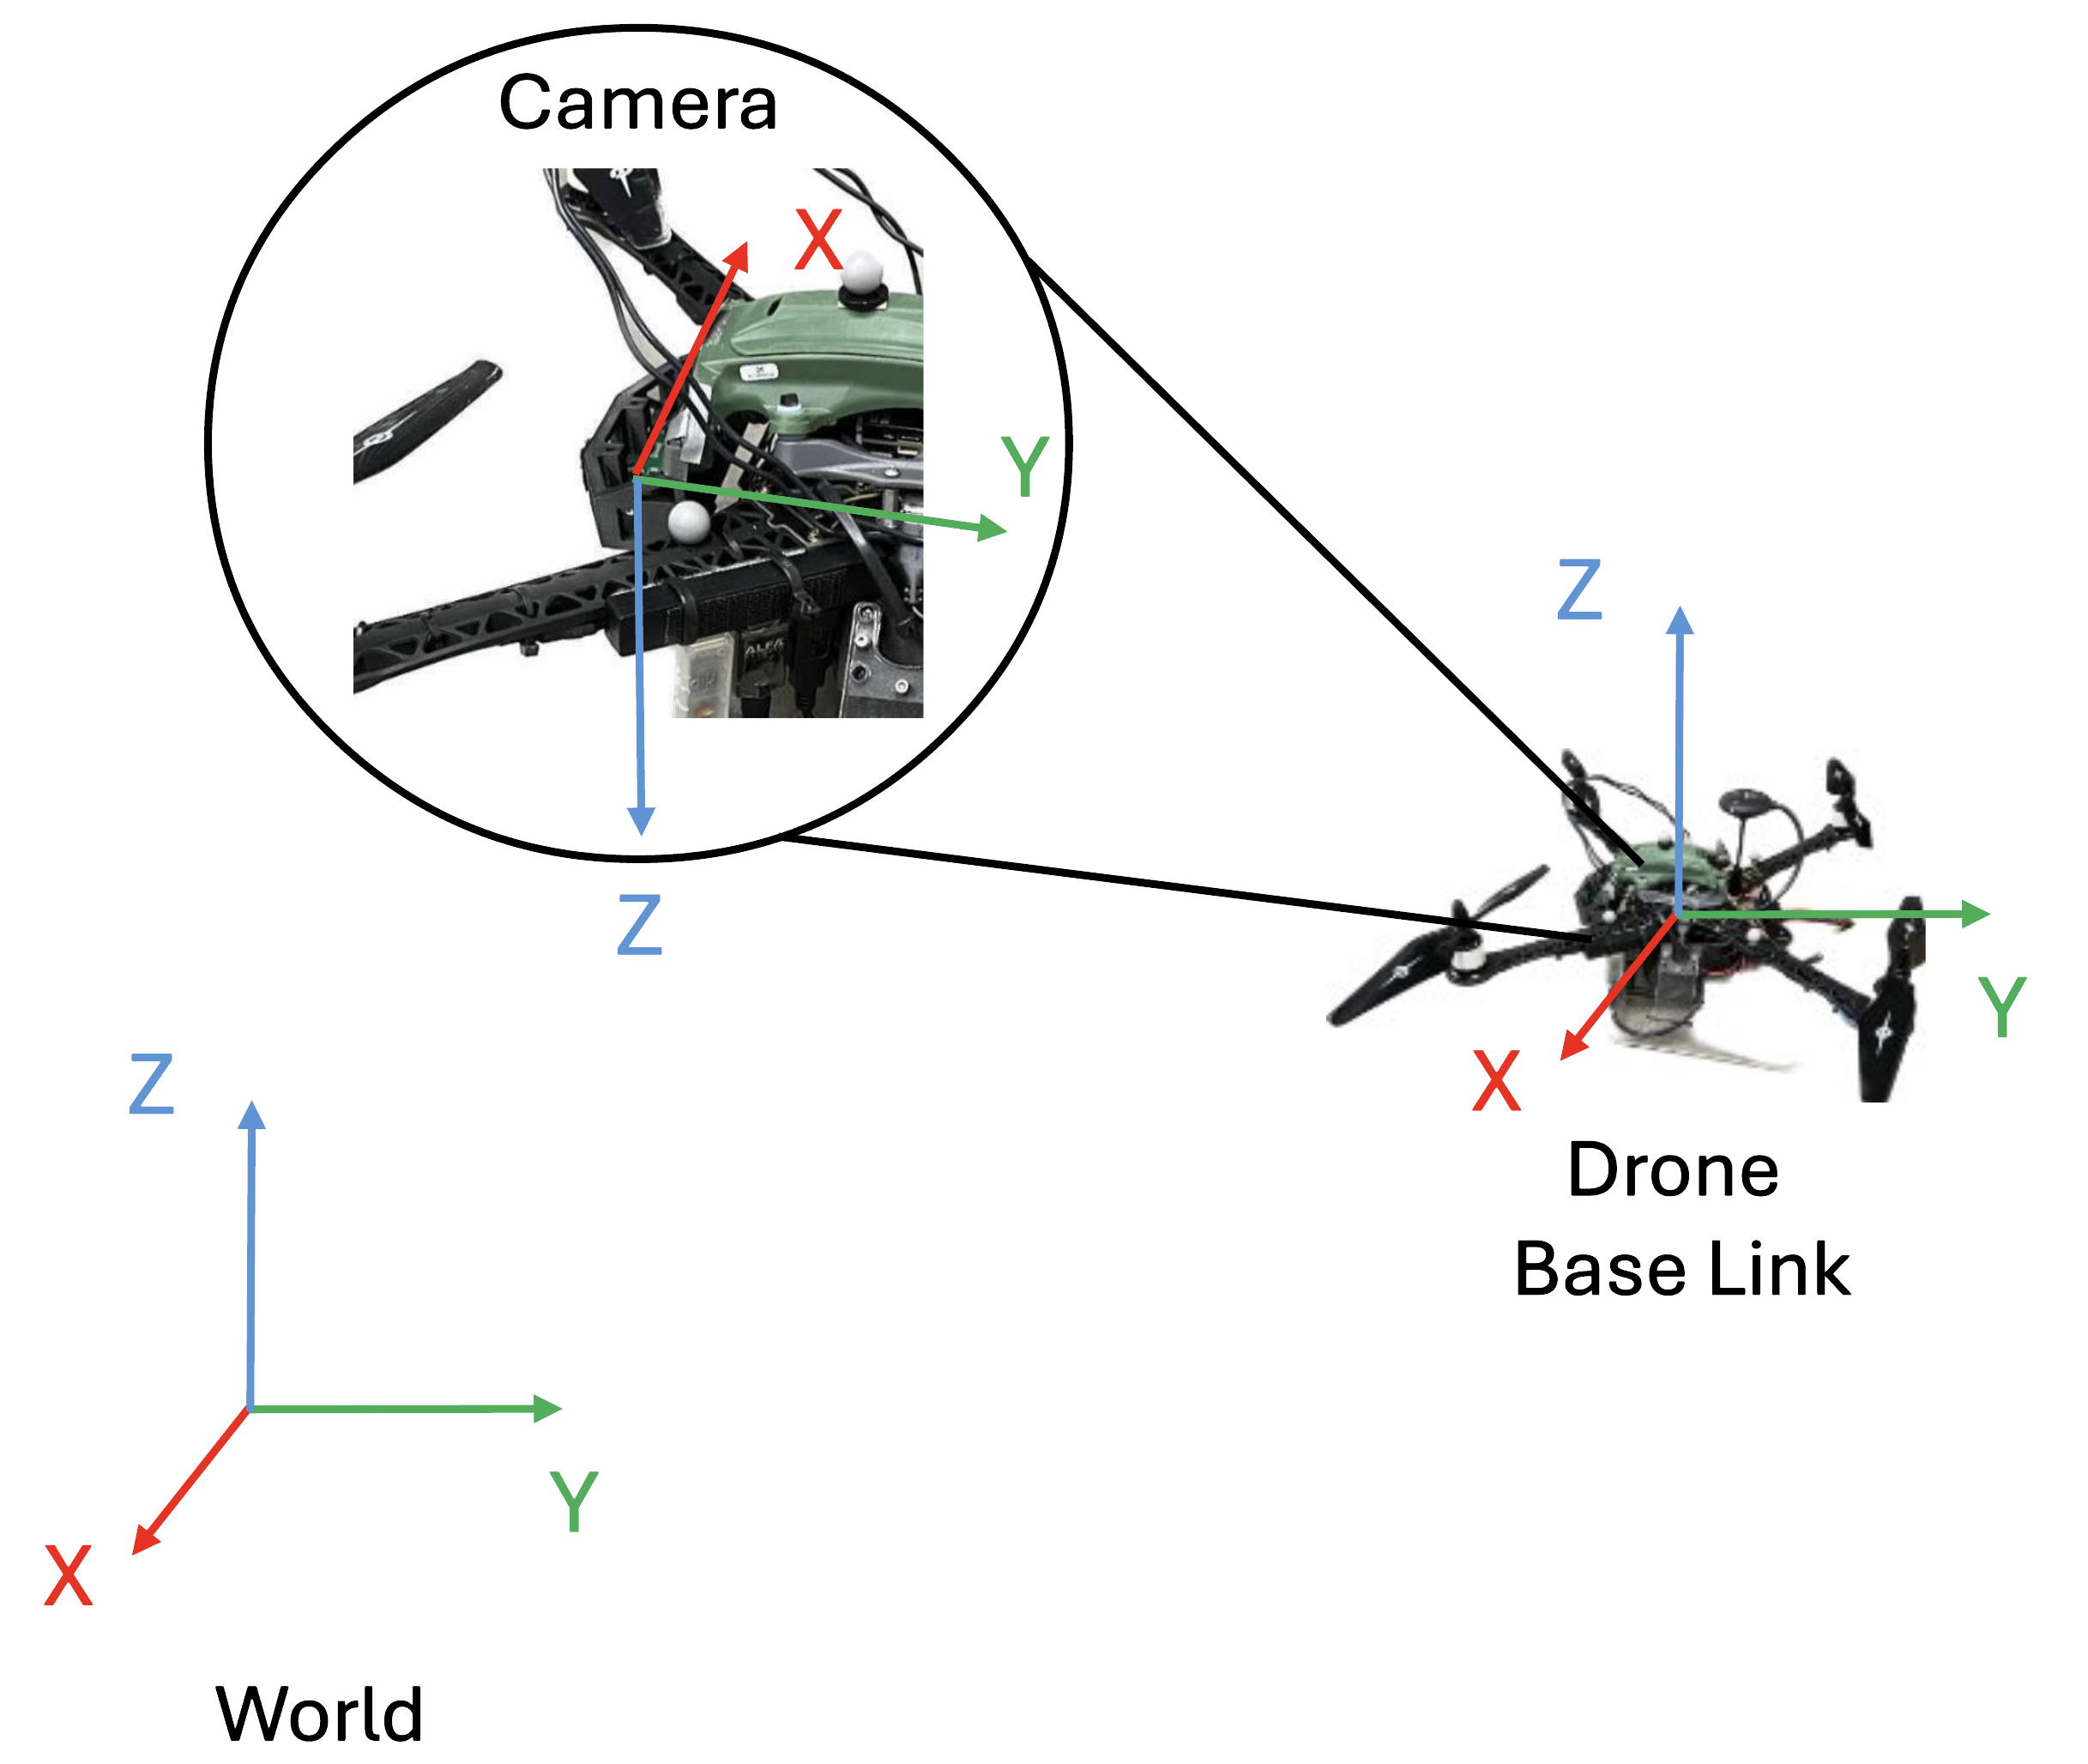
\includegraphics[scale=0.2]{images/stereo_camera_depth/frames.png}
\caption{Coordinate frames in stereo camera depth setup}
\label{fig:frames}
\end{figure}

Notably, there are three important frames:

\begin{itemize}
    \item The reference world frame $W$

    This is the global frame relative to which the drone flies, and the point clouds are created.

    \item The drone (base link frame) $D$
    
    This is the pose of the moving drone throughout a mission. It is constantly published by the simulation.

    \item The camera pose $C$
    
    The camera pose is the frame in which the point cloud is created and aggregated. The relative pose of the cameras is set in the simulated drone's setup file. This transformation is static and is applied to each incoming pose message directly.
\end{itemize}

Hereafter, the following notation is used:

\begin{itemize}
    \item $t_{dc}^W$: Transformation from drone to camera, represented in the World frame
    \item $R_{DC}$: Active Rotation from the Drone to the Camera frame
    \item $r_{wp}^W$: Position vector from the world frame to the detected point, represented in the World frame.
\end{itemize}

One more thing to note in \cref{fig:drone_sim_setup} is that in Gazebo's camera convention, the optical axis of a camera points along the x-axis. Therefore, the base link pose was subscribed to and converted to the camera pose using the respective transformation. Neither Gazebo's base link nor camera coordinate conventions are relevant as long as we correctly track the pose of a downwards-facing camera with the correct convention.

\subsection{Input Handling}
The input of the images and the base link pose are received using ROS subscribers. Despite publishing these simulated Gazebo topics at equal rates, they did not arrive simultaneously. In the completed setup using SFM this is handled by supplying SFM with both the image and the pose from the xVIO state estimator. As stereo needs two images from the stereo camera, this will have to be handled manually either by making xVIO also publish the stereo images or having some other way to ensure a synchronized delivery of the stereo images and the xVIO pose.

The pose is only required for transferring the created points from the camera frame to the world frame. Therefore, the two input images were processed into a depth image in a single step, and only then were all three inputs used together to create the point cloud. 

\cref{fig:input_synch} schematically shows how the stereo camera depth node handled this shortcoming of asynchronous sensor messages by manually picking the pose which temporally closest corresponds to the image's timestamp. This was possible as the image processing step dominates the computation time of the input handling, and the pose can thus be updated in the meantime to best fit the image timestamps.

\clearpage %HERE

\begin{figure}[h]
\centering
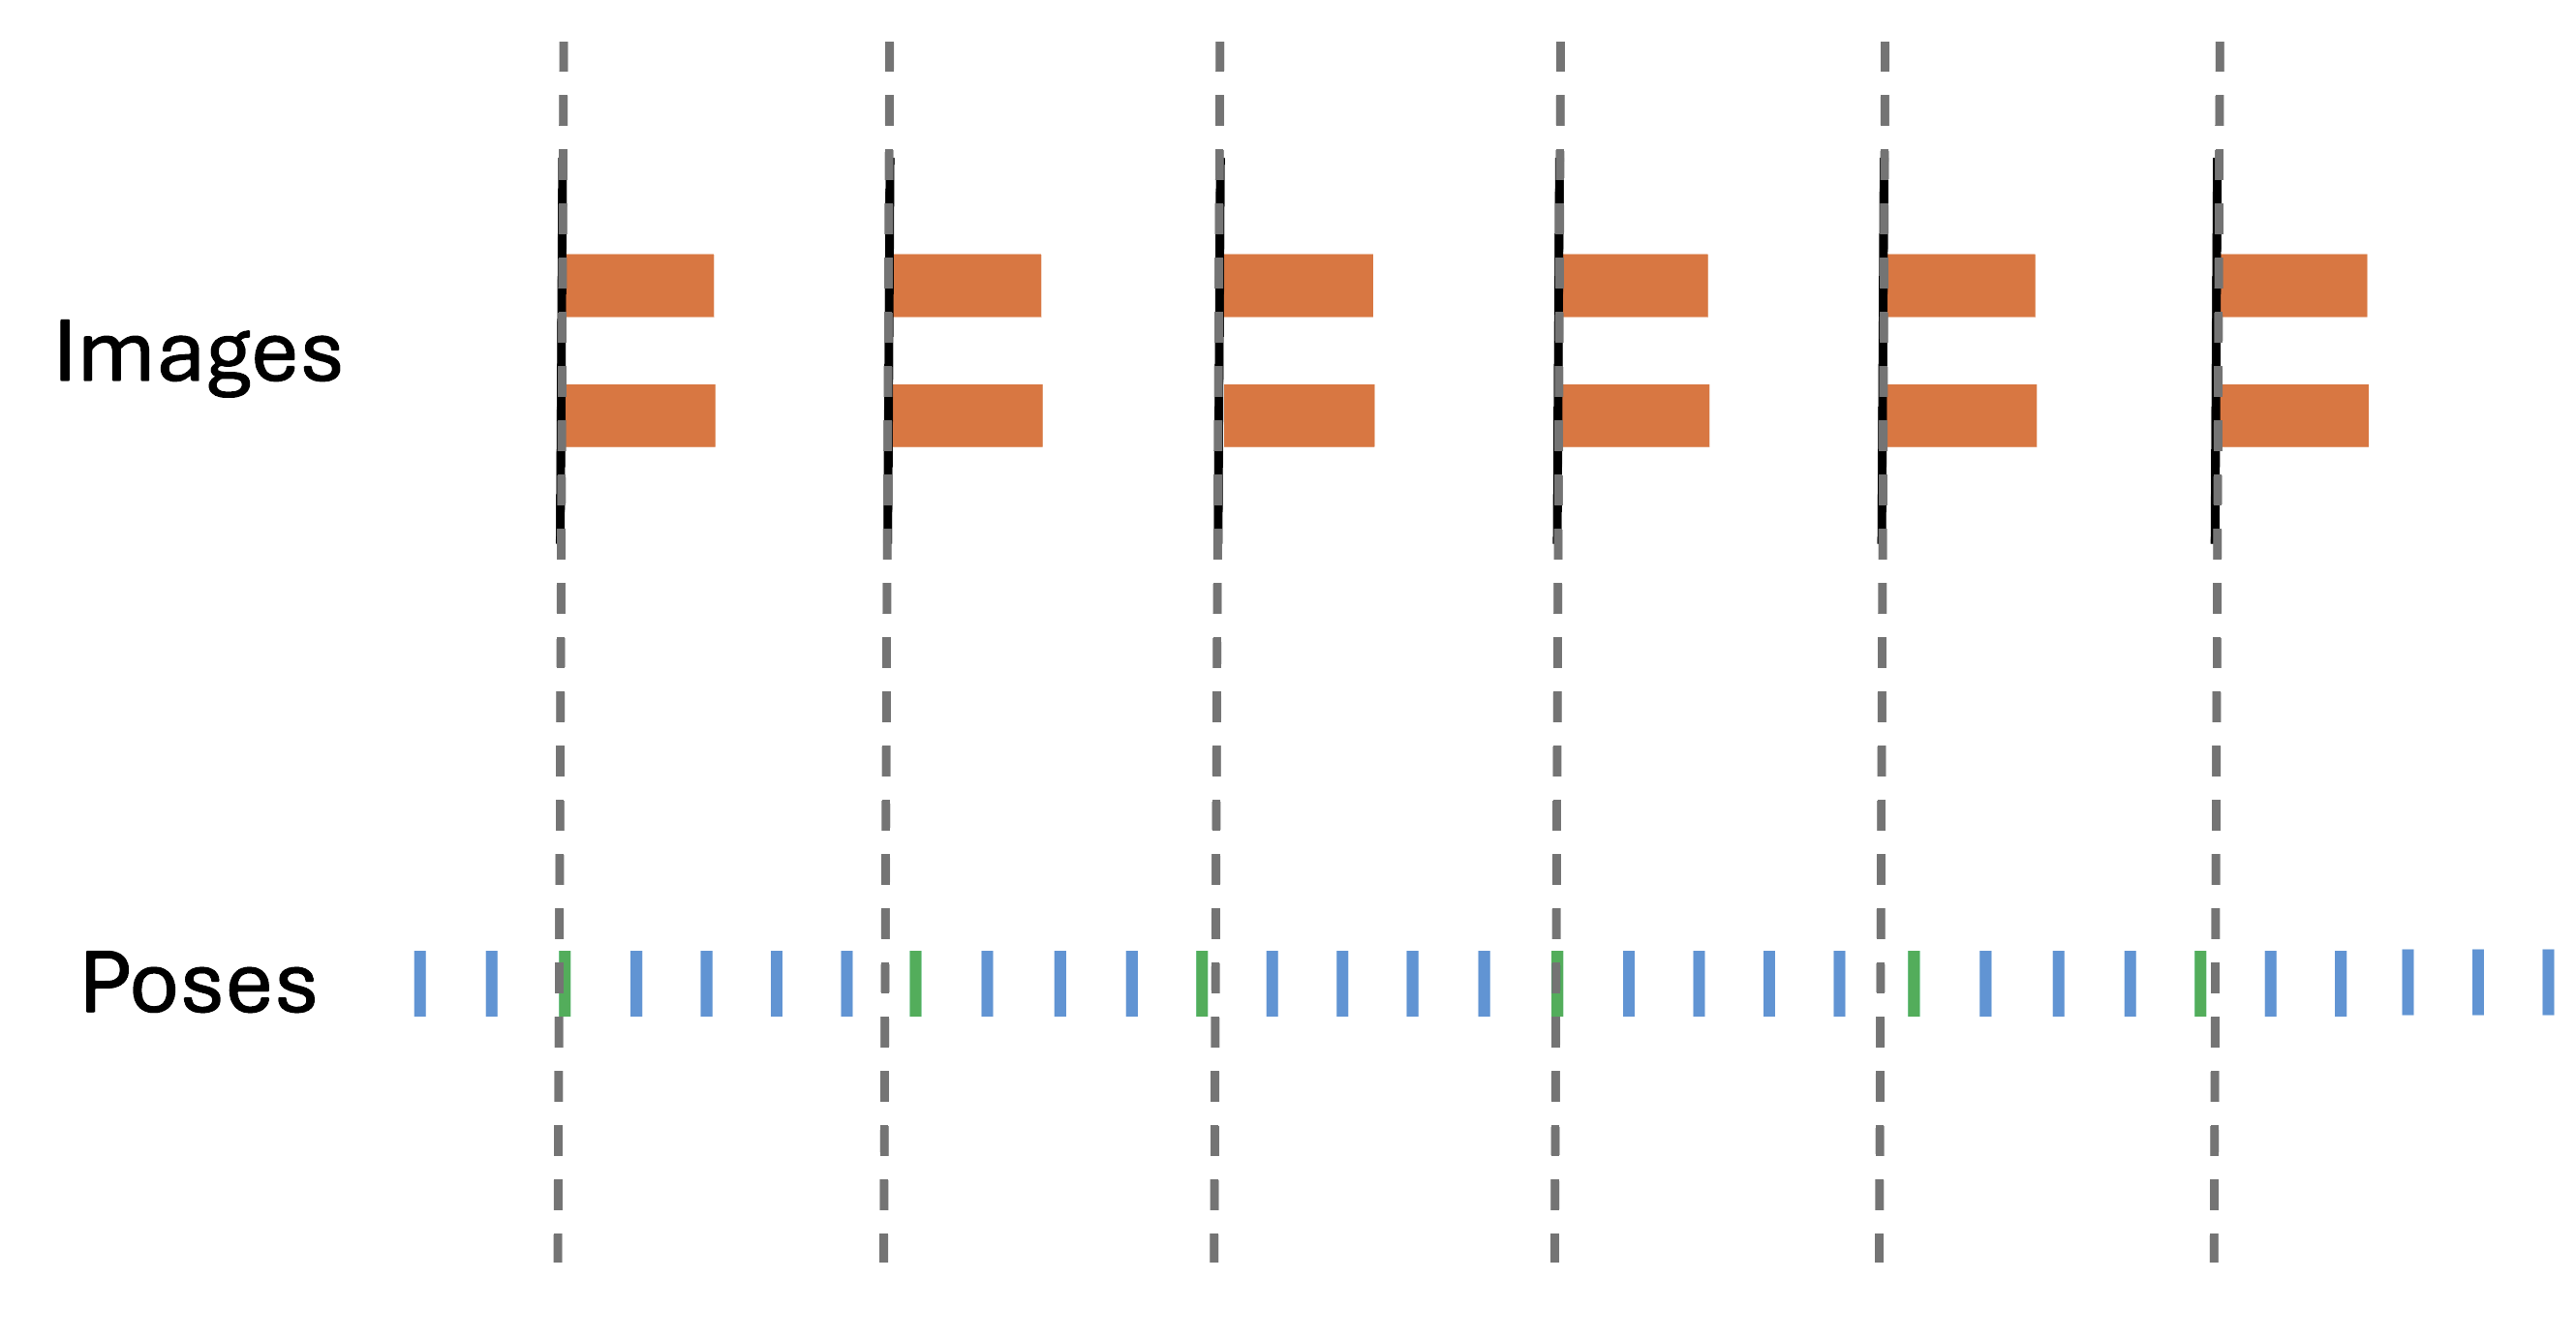
\includegraphics[scale=0.26]{images/stereo_camera_depth/input_synchronization.png}
\caption{Schematic visualization of input synchronization used in the stereo depth node}
\label{fig:input_synch}
\end{figure}

\subsection{Disparity Creation}\label{subsec:disparity_creation}

The chosen StereoSGBM (Semi-Global Block Matching) algorithm creates a disparity map from two horizontally aligned images using an approach based on Heiko Hirschmüller's stereo approach introduced in \citep{Stereo}. 

The resulting disparity image is shown in \cref{fig:stereo_disp}.

\begin{figure}[h]
\centering
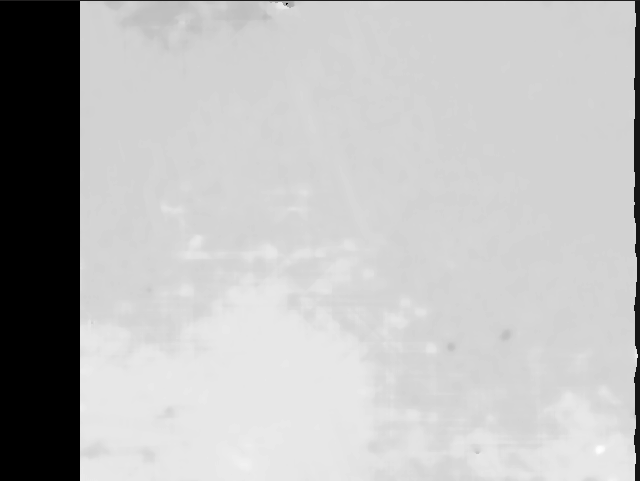
\includegraphics[scale=0.5]{images/stereo_camera_depth/stereo_disparity.png}
\caption{Disparity image from the stereo camera using StereoSGBM.}
\label{fig:stereo_disp}
\end{figure}

The StereoSGBM algorithm cuts off the left boundary, as can be seen in \cref{fig:stereo_disp}. This is due to the maximum disparity parameter, which prevents the pixels on the left border of the left image from being matched. As the left image is the reference image, the output removes the border. Additionally, artifacts could be seen on the right-hand side of the image. Both of these border artifacts were filtered out using a mask.

\subsection{Point Cloud Creation}

Having created a disparity image using the approach laid out in \cref{subsec:disparity_creation}, the disparity pixels are first converted to the depth values using the classic disparity depth relation \ref{eq:depth_from_disp} shown in \cref{subsec:theoretical_analysis}.

\begin{figure}[h]
\centering
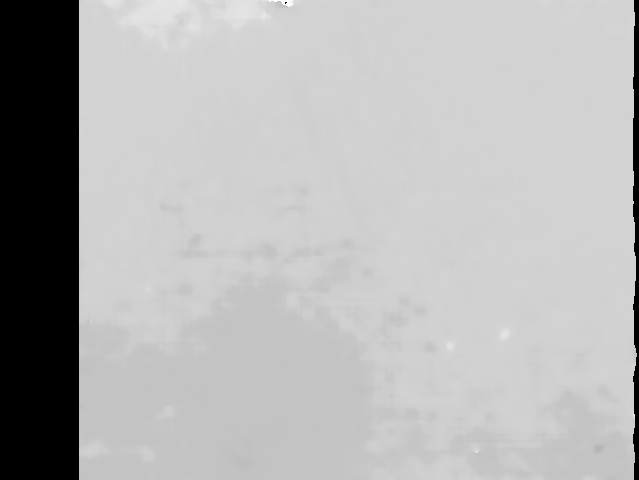
\includegraphics[scale=0.5]{images/stereo_camera_depth/stereo_depth.png}
\caption{Stereo depth image}
\label{fig:stereo_depth}
\end{figure}

The 3D locations of each detected point can be derived from the created depth image, pose, and camera parameters. This is done by simply tracing the projection line of the detected point as indicated in \cref{fig:line_projection} and using the similar triangles as shown in \cref{fig:similar_triangles}

\begin{figure}[h]
\centering
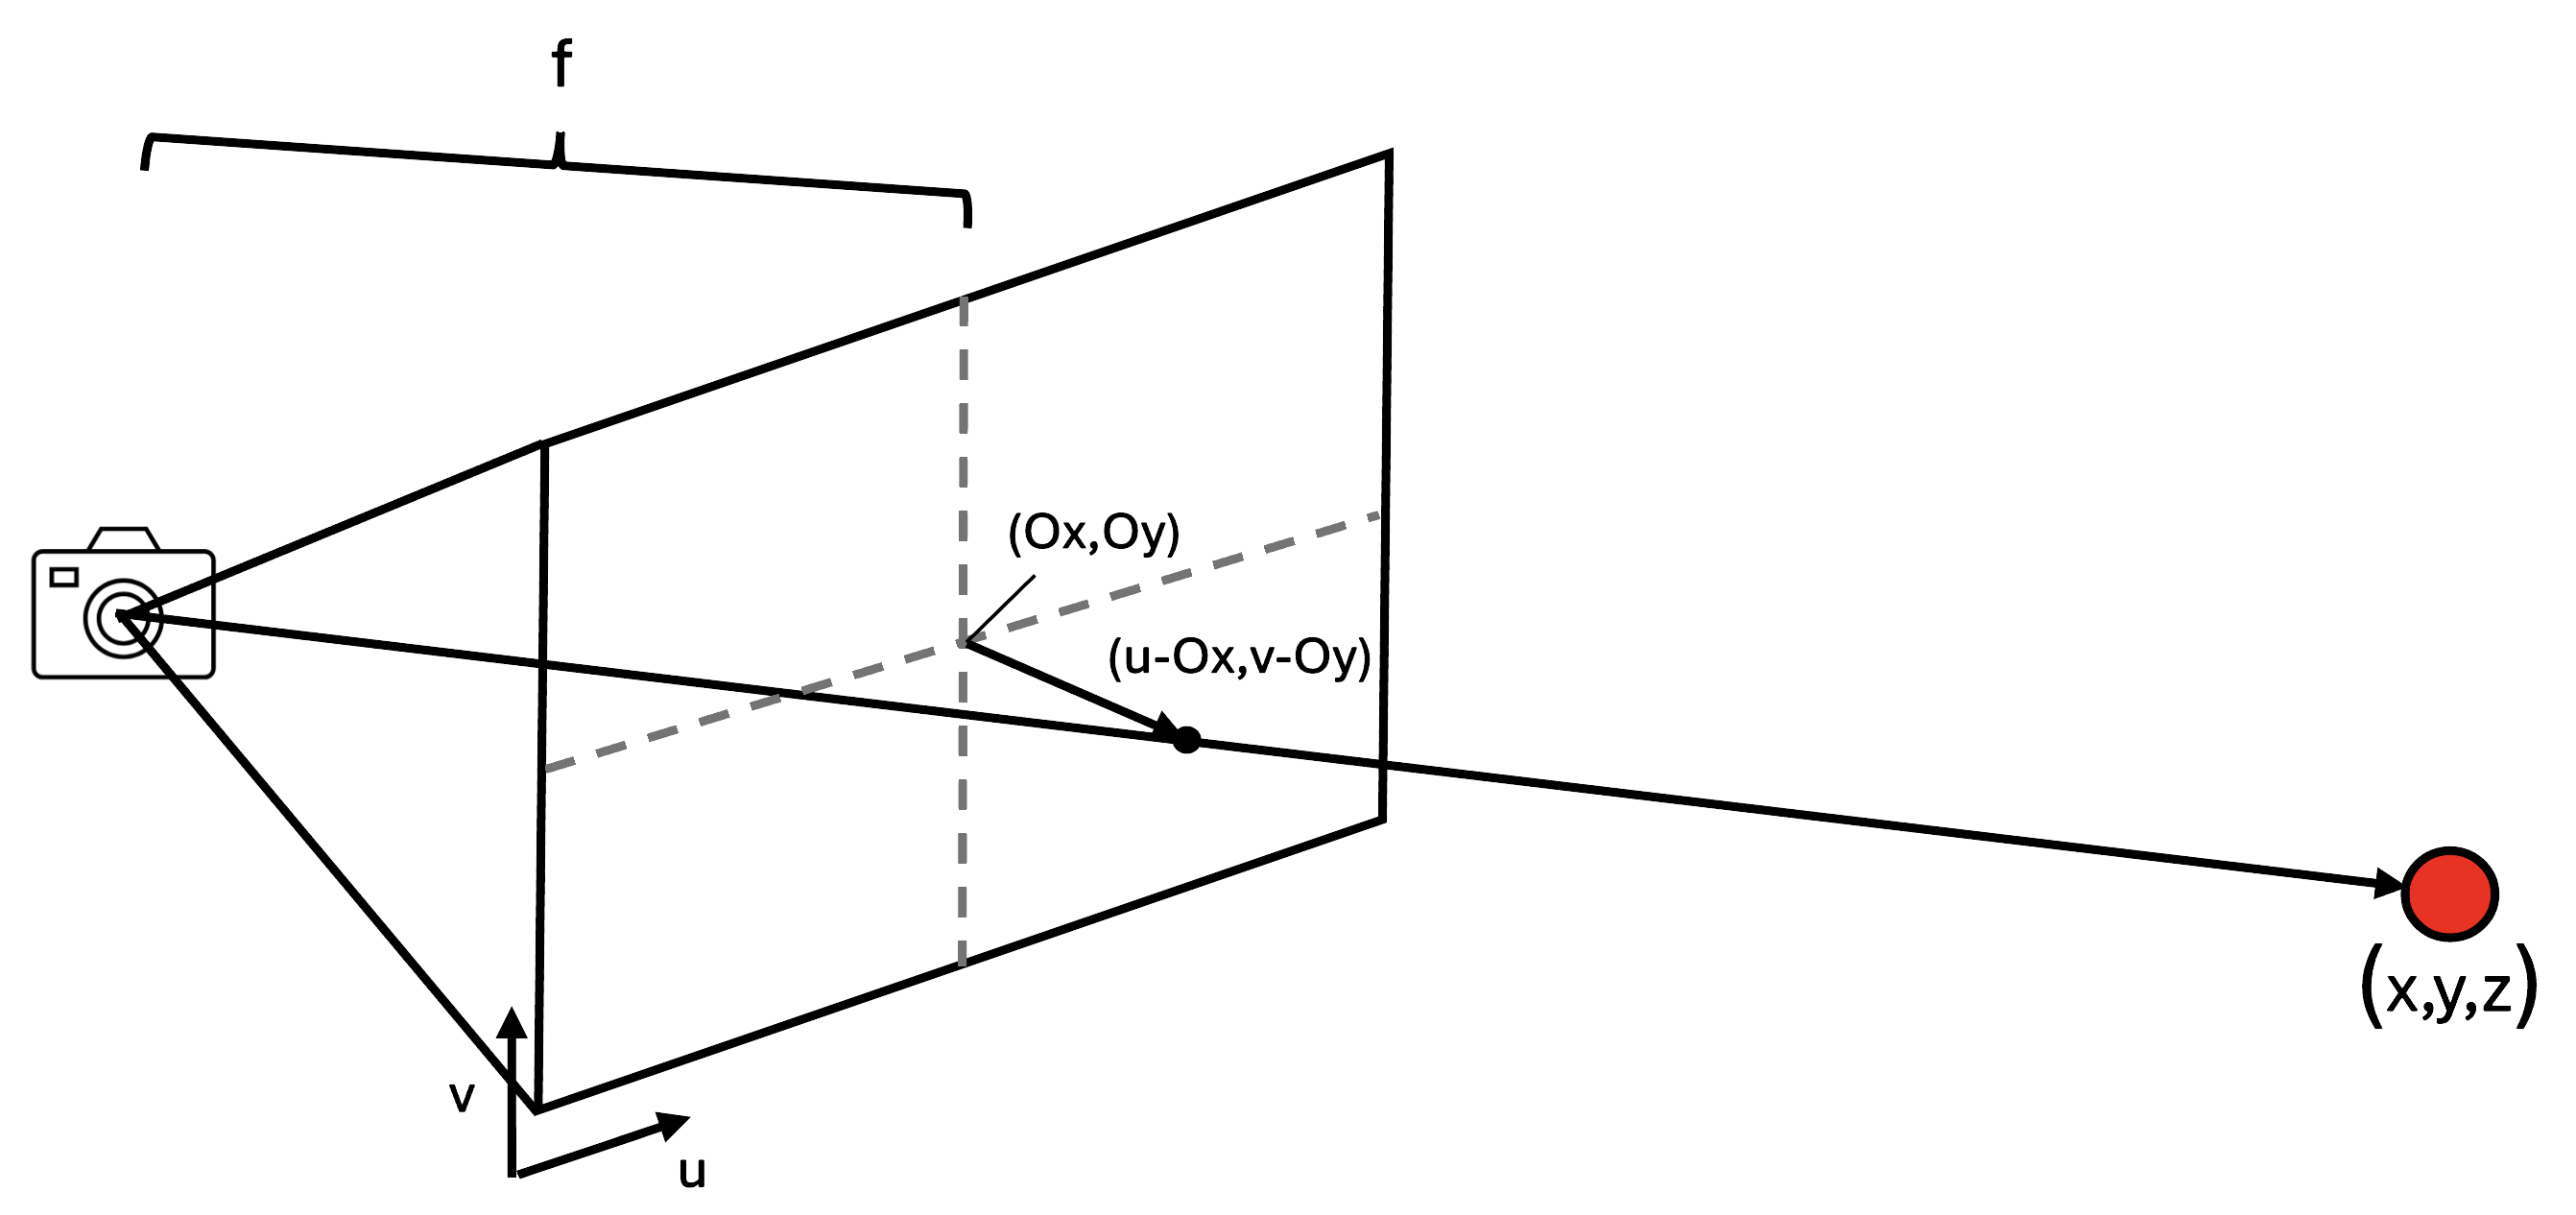
\includegraphics[scale=0.25]{images/stereo_camera_depth/projection.png}
\caption{Schematic of the line projection procedure to derive the 3D location of detected points}
\label{fig:line_projection}
\end{figure}

\begin{figure}[h]
\centering
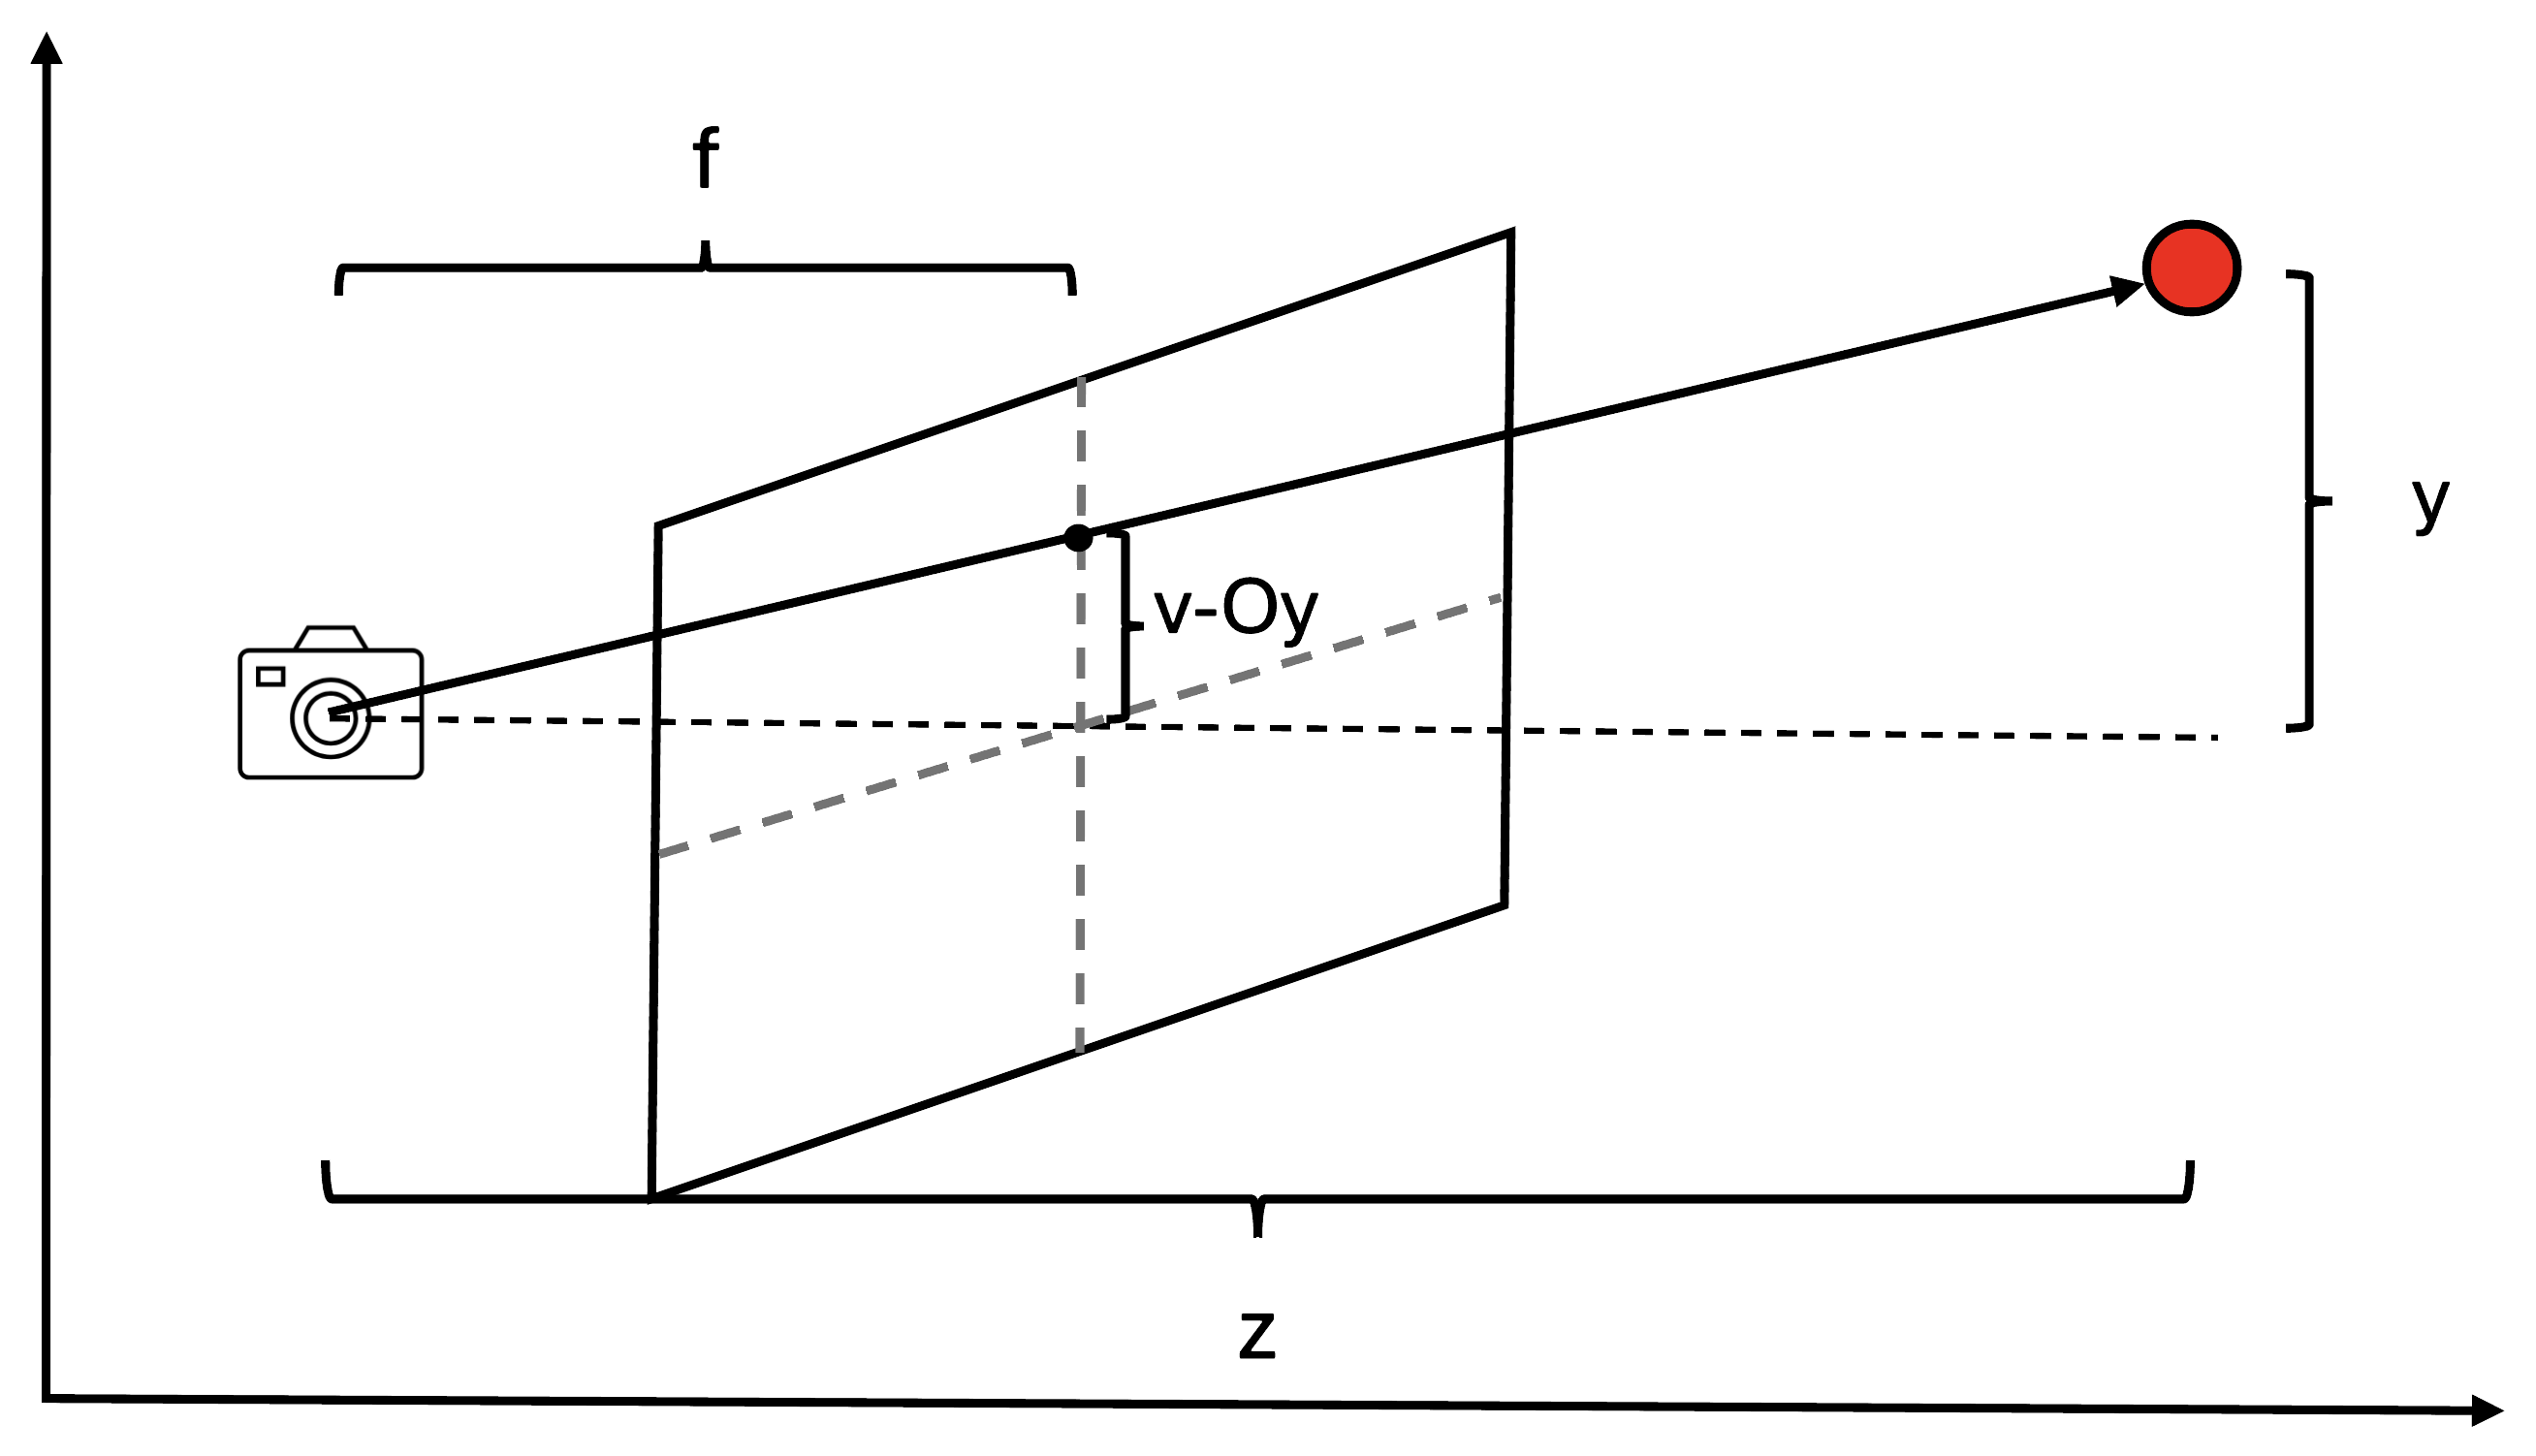
\includegraphics[scale=0.25]{images/stereo_camera_depth/similar_triangles.png}
\caption{Schematic of the line projection procedure to derive the 3D location of detected points}
\label{fig:similar_triangles}
\end{figure}

The formulas for the point coordinates in the camera frame are shown in \cref{eq:pc_projection}.

\begin{align}
    \label{eq:pc_projection}
    x_{cp}^C &= \text{depth} * \frac{\left(u - o_x\right)}{f_x}\\
    y_{cp}^C &= \text{depth} * \frac{\left(v - o_y\right)}{f_y}\\
    z_{cp}^C &= \text{depth} \quad \text{Depth value is the same}
\end{align}

Lastly, to get the point cloud in the world frame, the coordinate transform is applied:

\begin{align}
    r_{wp}^W &= r_{wc}^W + R_{WC} \cdot r_{cp}^C\\
             &= r_{wd}^W + R_{WD} \cdot r_{dc}^D + R_{WC} \cdot r_{cp}^C
    \label{eq:transform_CW}
\end{align}

Where

\begin{equation}
    r_{cp}^C = \begin{pmatrix}
        x_{cp}^C\\
        y_{cp}^C\\
        z_{cp}^C
    \end{pmatrix}
    \label{eq:camera_point_vector}
\end{equation}

The final point cloud created using this process is shown in \cref{fig:stereo_pc}.

\begin{figure}[h]
\centering
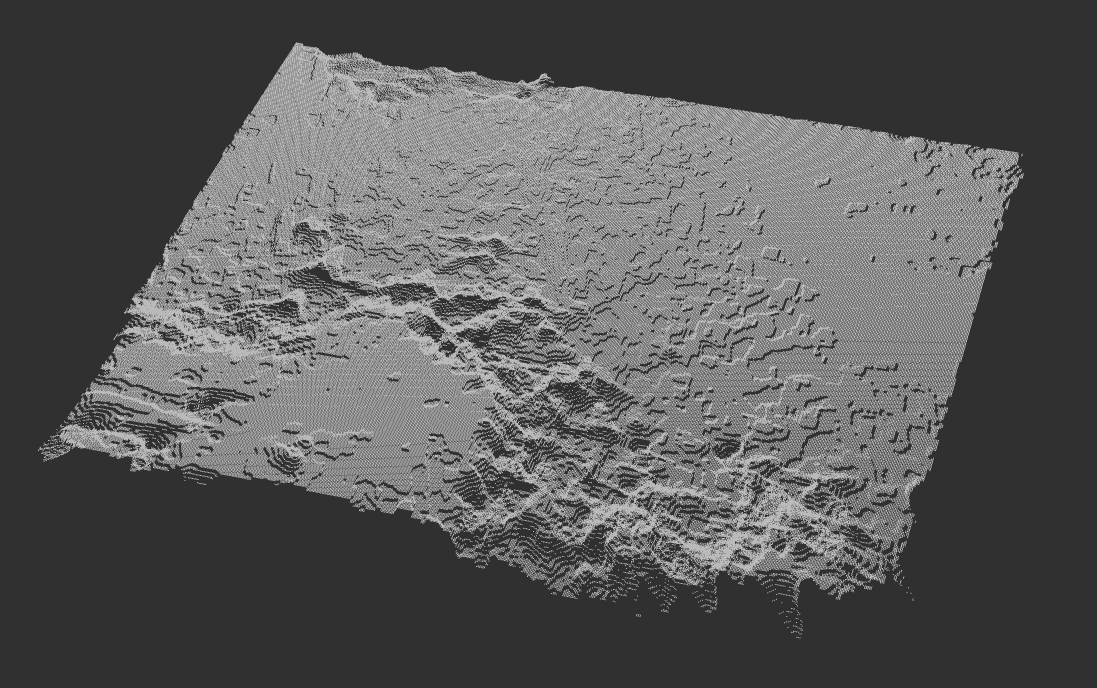
\includegraphics[scale=0.3]{images/stereo_camera_depth/stereo_pc.png}
\caption{RViz visualization of stereo camera point cloud}
\label{fig:stereo_pc}
\end{figure}

The node's final output is a point cloud generated in the world frame, together with two poses representing the camera locations of the generated point cloud.

\clearpage %HERE

% \subsubsection{StereoSGBM vs StereoBM}\label{subsec:bmvssgbm}

% Apart from the StereoSGBM implementation, OpenCV provides the StereoBM algorithm, which is generally faster but less precise.

% Implementing and comparing the two algorithms, the following results were seen:

% \begin{figure}[h]
% \centering
% 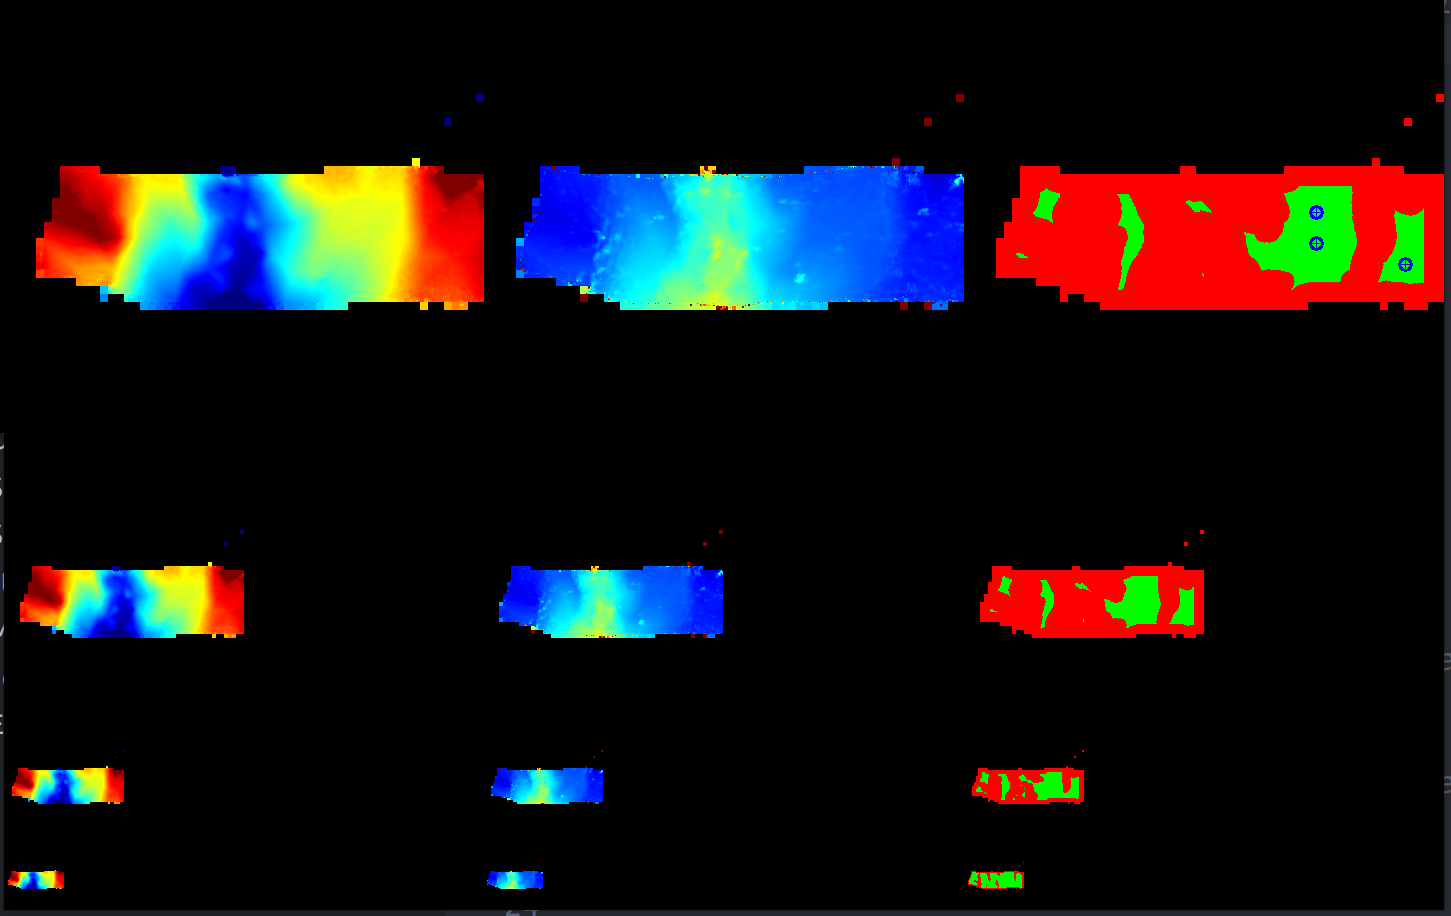
\includegraphics[scale=0.23]{images/stereo_camera_depth/stereoBM.png}
% \caption{LSD debug image when using the StereoBM algorithm}
% \label{fig:stereoBM}
% \end{figure}

% \begin{figure}[h]
% \centering
% 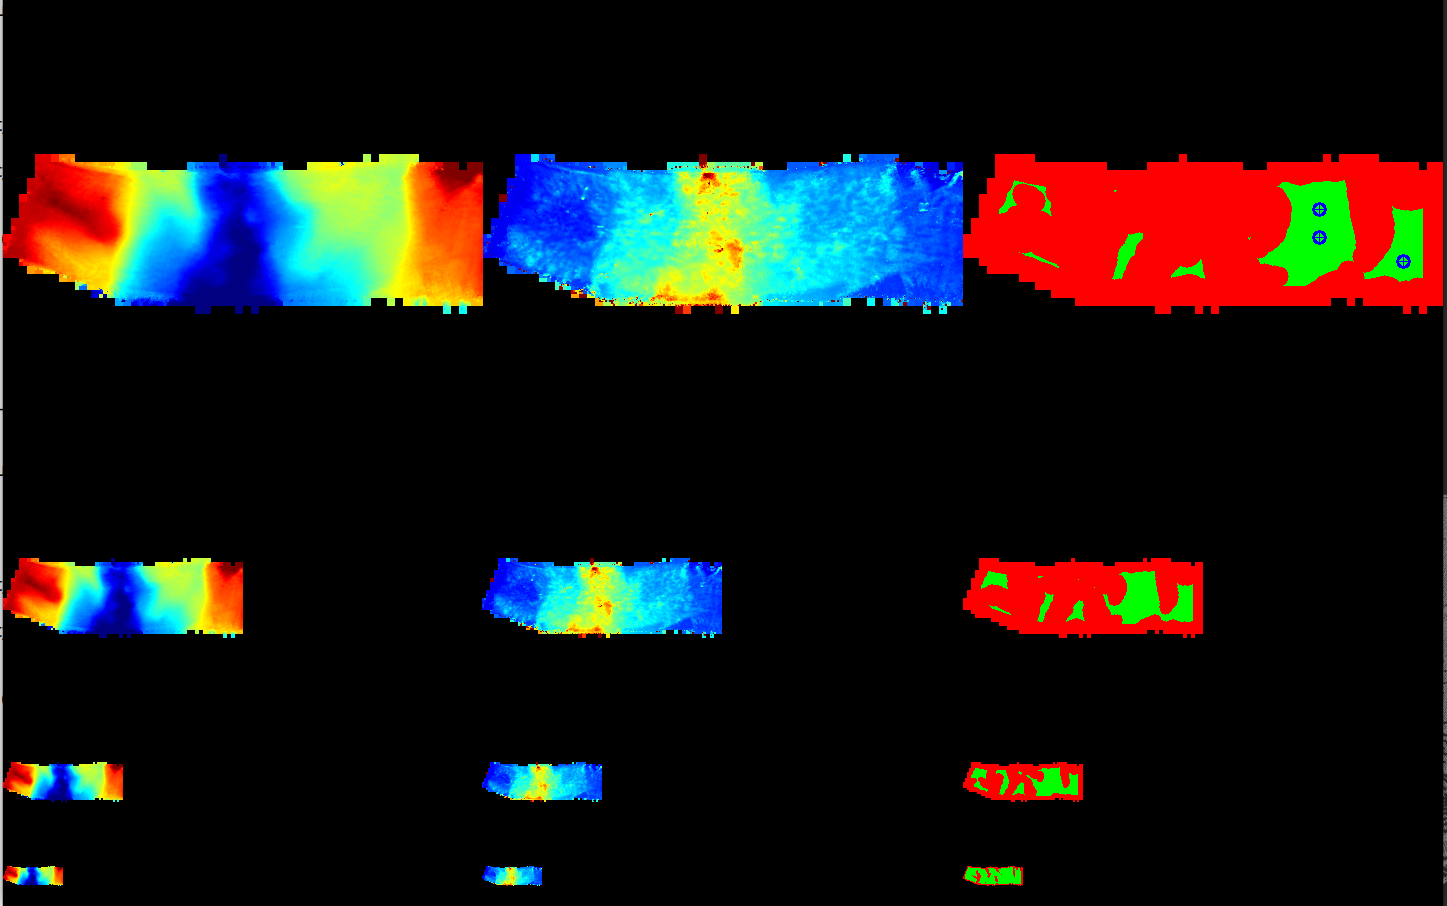
\includegraphics[scale=0.23]{images/stereo_camera_depth/stereoSGBM.png}
% \caption{LSD debug image when using the StereoSGBM algorithm}
% \label{fig:stereoSGBM}
% \end{figure}

% As can be seen in the figures \cref{fig:stereoBM} and \cref{fig:stereoSGBM}, StereoBM did not, in general, perform badly. However, quite regularly, StereoBM produced erroneous points. In general, a swift algorithm like StereoBM is preferable for our purposes. Nevertheless, precise terrain reconstruction is a vital pipeline component; thus, the quality must not be compromised. Therefore, StereoSGBM remained the algorithm for stereo depth creation.
% \clearpage %HERE

\subsection{Switching}\label{subsec:switching}

One needs to switch between the two alternatives to achieve the final desired perception mechanism of flying laterally with SFM and using a stereo camera depth node at low altitudes.

The drone's current altitude above ground is the obvious decision boundary to implement in the switching mechanism. This could be achieved by analyzing the generated point cloud at a given iteration to determine the median altitude, which indicates the altitude above ground. However, this is an avoidable computational overhead.

As mentioned in \cref{sec:sys_overview}, the drone has a laser range finder on board. This allows us to estimate the altitude above ground at any given moment without needing image processing.

Therefore, the switching is performed using a separate ROS subscriber, which continuously checks the LRF's measurement and activates or deactivates the SFM node and stereo node, respectively. This is schematically shown in \cref{fig:switching}.\footnote[1]{BG image source: Adobe Stock images
% \href{https://www.google.com/url?sa=i&url=https%3A%2F%2Fstock.adobe.com%2Fsearch%3Fk%3Dmars%2Bground&psig=AOvVaw2EEFVKYMdr4tWB3kzVOCwz&ust=1719217248402000&source=images&cd=vfe&opi=89978449&ved=0CBEQjRxqFwoTCNius76l8YYDFQAAAAAdAAAAABAE}
}

\begin{figure}[h]
    \centering  
    \includegraphics[scale=0.17]{images/stereo_camera_depth/switching.png}
    \caption{Laser Ranger Finder Based Switch between Depth Sources}
    \label{fig:switching}
\end{figure}

A second application of this switching is to disable the stereo node until the drone reaches approximately 50 cm altitude. The reason for this is that the camera images don't have sufficient overlap to detect matches for the closest points with the largest disparities below that altitude. This is because the StereoSGBM algorithm is implemented with a maximum disparity of 80 pixels. This is shown in \cref{fig:overlap}.

\clearpage %HERE

\begin{figure}[h]
    \centering
    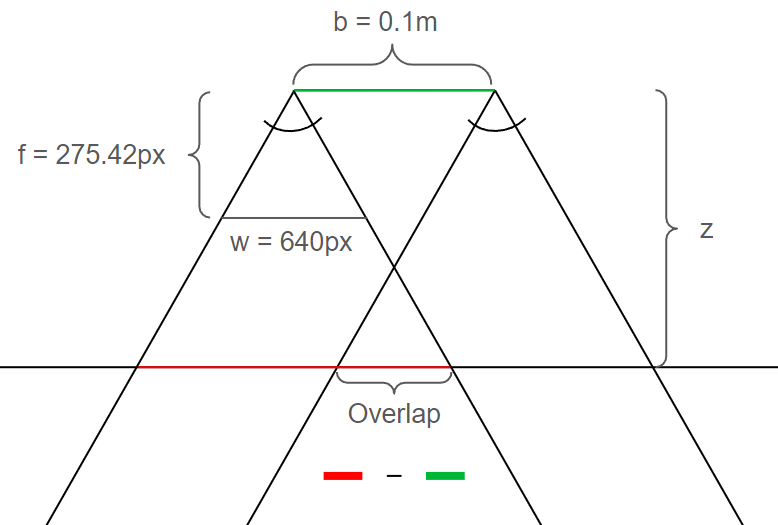
\includegraphics[scale=0.5]{images/stereo_camera_depth/overlap.png}
    \caption{Overlap problem at low altitudes: The baseline is indicated in green, and the image footprint in red. The overlap of the two camera images is the reference camera's image footprint minus the baseline.}
    \label{fig:overlap}
\end{figure}

With the given camera parameters shown in \cref{sec:stereo_methodology}, the metric image overlap is calculated to be.

\begin{equation}
    overlap = 2 \cdot \frac{w}{2\cdot f} \cdot z - b = \frac{w\cdot z}{f} - b = \frac{640\cdot z}{275.42} - 0.1 m
    \label{eq:overlap}
\end{equation}

\begin{equation}
    overlap = \frac{d \cdot z}{f} = \frac{80 \cdot z}{275.42}
    \label{eq:disp_overlap}
\end{equation}

\cref{eq:disp_overlap} shows the minimum image overlap required for a possible maximum disparity of 80 pixels. Plugging this into \cref{eq:overlap} and solving for z, we get:

\begin{equation}
    z = \frac{b \cdot f}{w - d} = \frac{0.1 m \cdot 275.42}{640 - 80} = 0.04918 m
\end{equation}

Therefore, the drone must be at least 50 cm in the air to perceive depth well. Note that this is rather a high minimum altitude. This is because the simulated cameras have rather small focal lengths. The trade-off with smaller focal lengths is the ability to use stereo higher above the ground. 

For instance, a camera pair with a focal length of 512 pixels and the otherwise same setup would only need a minimum altitude of 9.14 cm. However, the altitude at which a depth error of 10 cm is already at  2.347 m as opposed to the derived
3.184 m shown in \cref{fig:stereo_limit}.

\subsection{Landing Site Detection without Lateral Motion}

Taking off vertically with the drone in the simulation, the first landing site in the LORNA project without lateral motion was found. \cref{fig:vertical_ls_sim}, \cref{fig:vertical_ls_pc}, and \cref{fig:vertical_ls_lsd} show the drone in the simulation, the generated stereo point cloud and the landing site detected in the LSD debug image respectively.

\begin{figure}
    \centering
    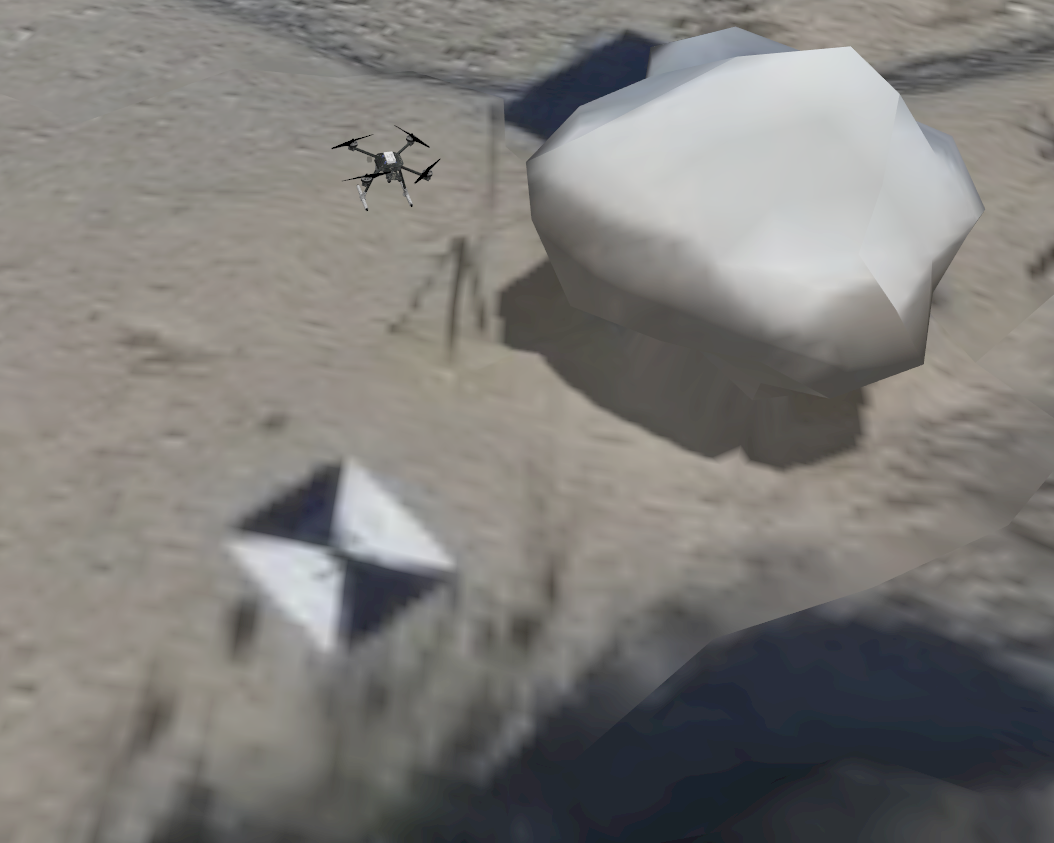
\includegraphics[scale=0.34]{images/stereo_camera_depth/ascent_sim.png}
    \caption{Drone during vertical ascent in simulation}
    \label{fig:vertical_ls_sim}
\end{figure}

\begin{figure}
    \centering
    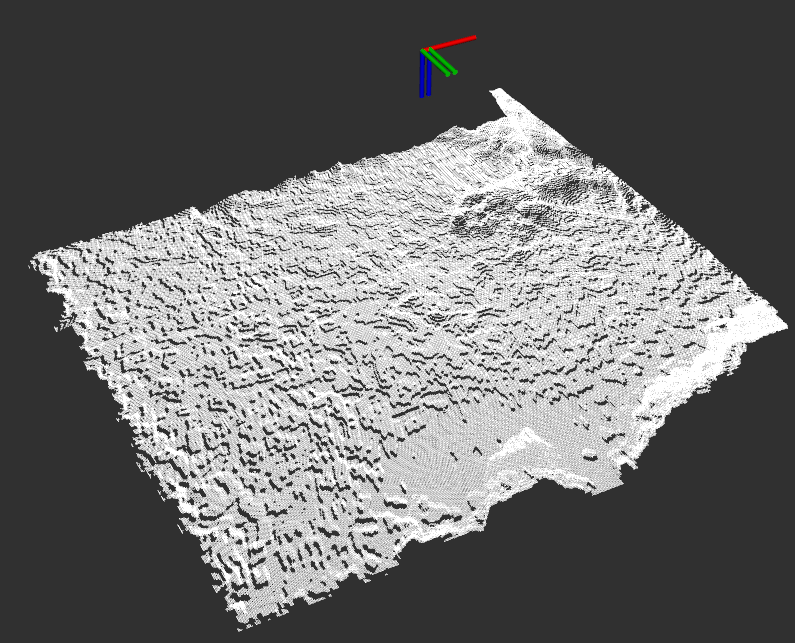
\includegraphics[scale=0.45]{images/stereo_camera_depth/stereo_pointcloud.png}
    \caption{RViz visualization of created point cloud from stereo camera}
    \label{fig:vertical_ls_pc}
\end{figure}
\clearpage %HERE

\begin{figure}
    \centering
    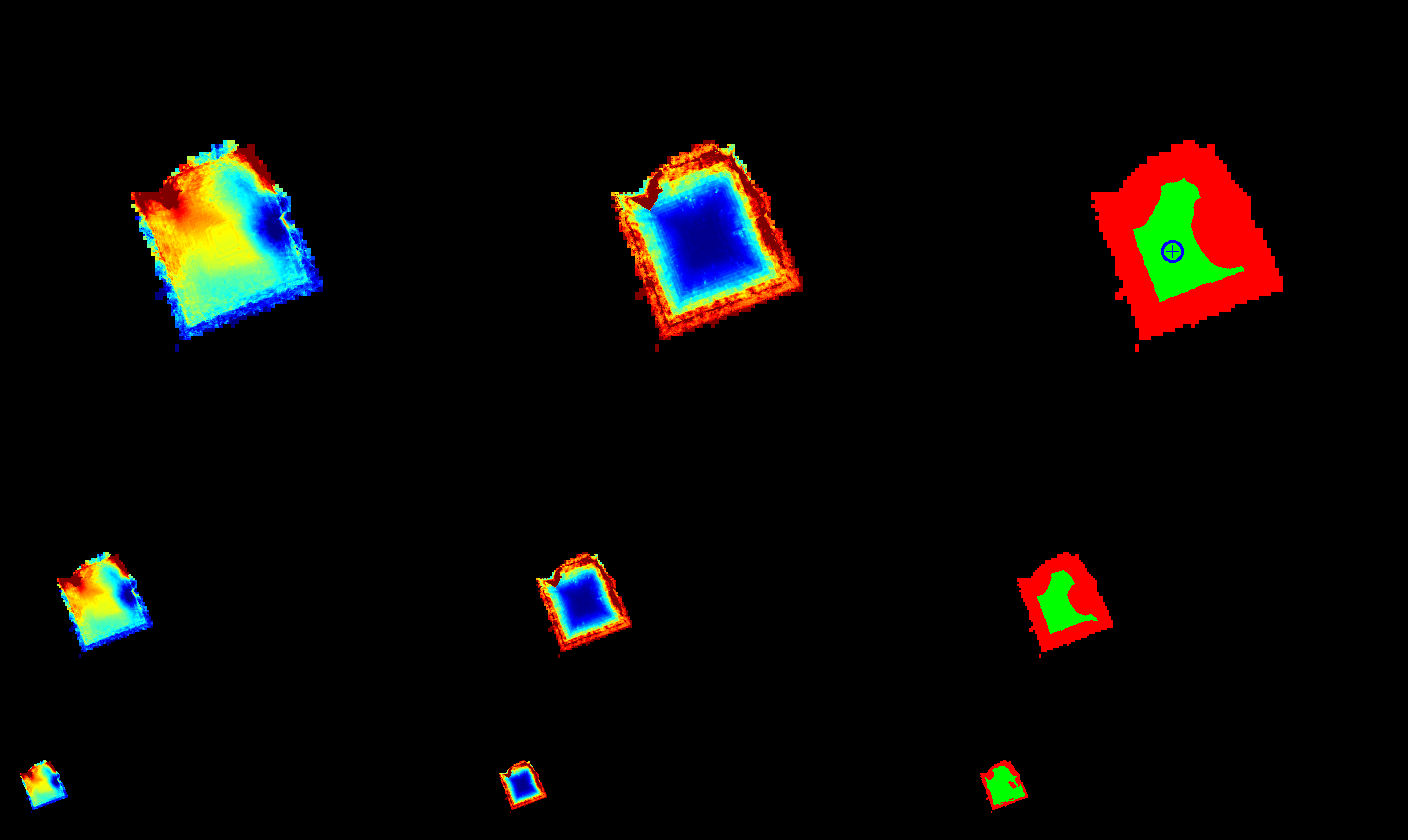
\includegraphics[scale=0.25]{images/stereo_camera_depth/lsd_ascent.png}
    \caption{LSD Debug output displaying LORNA's first detected landing site during vertical motion}
    \label{fig:vertical_ls_lsd}
\end{figure}

\section{Qualitative Practical Analysis}

Once implemented, the landing site detection instance could be supplied by the stereo depth node. The result thereof can be seen below:

\begin{figure}[ht!]
    \centering
    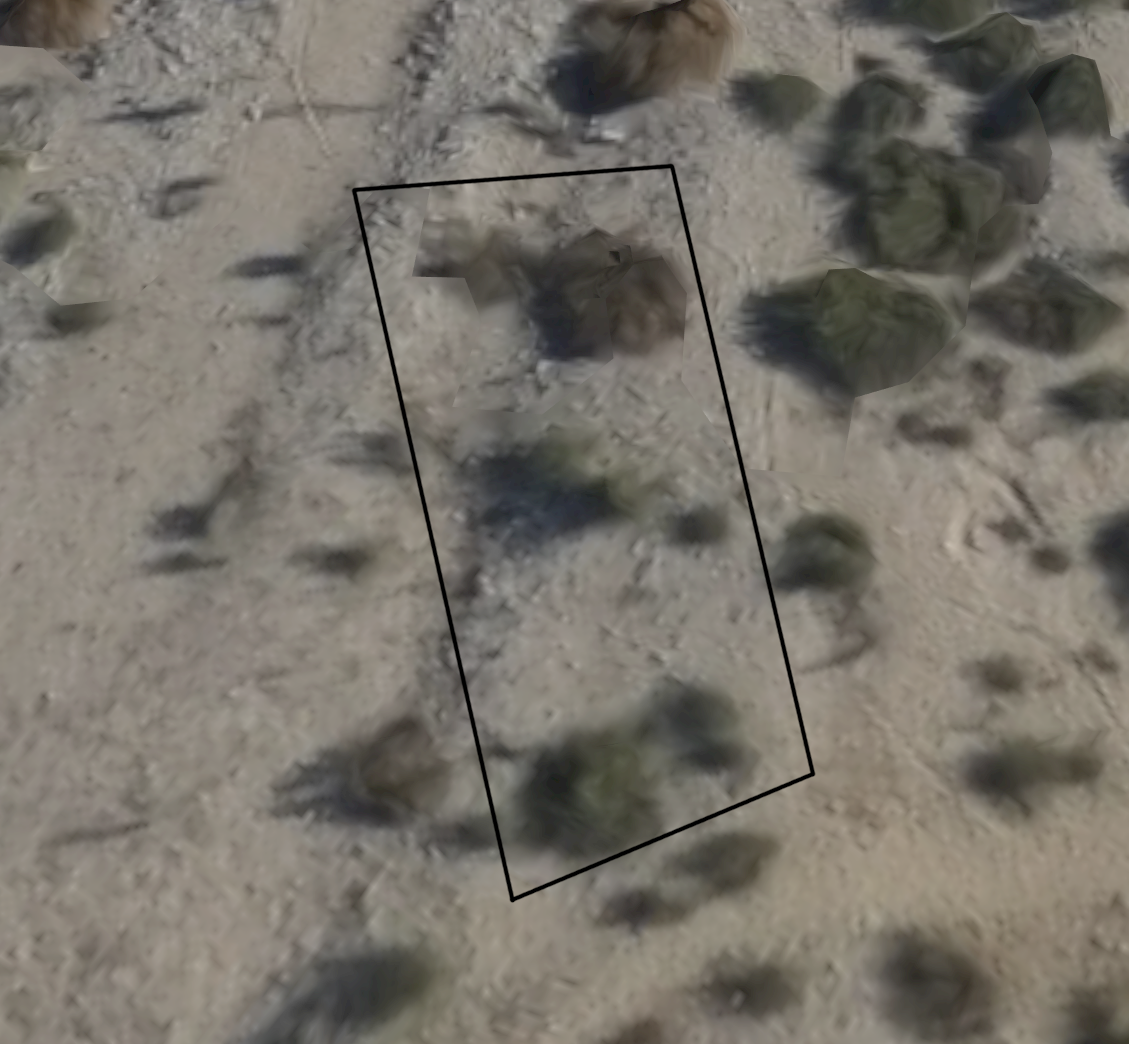
\includegraphics[scale=0.2, angle=-12]{images/stereo_camera_depth/reference_map2.5m_annotated.png}
    \caption{Considered terrain patch in Gazebo simulation}
    \label{stereo_reference}
\end{figure}

\begin{figure}[ht!]
    \centering
    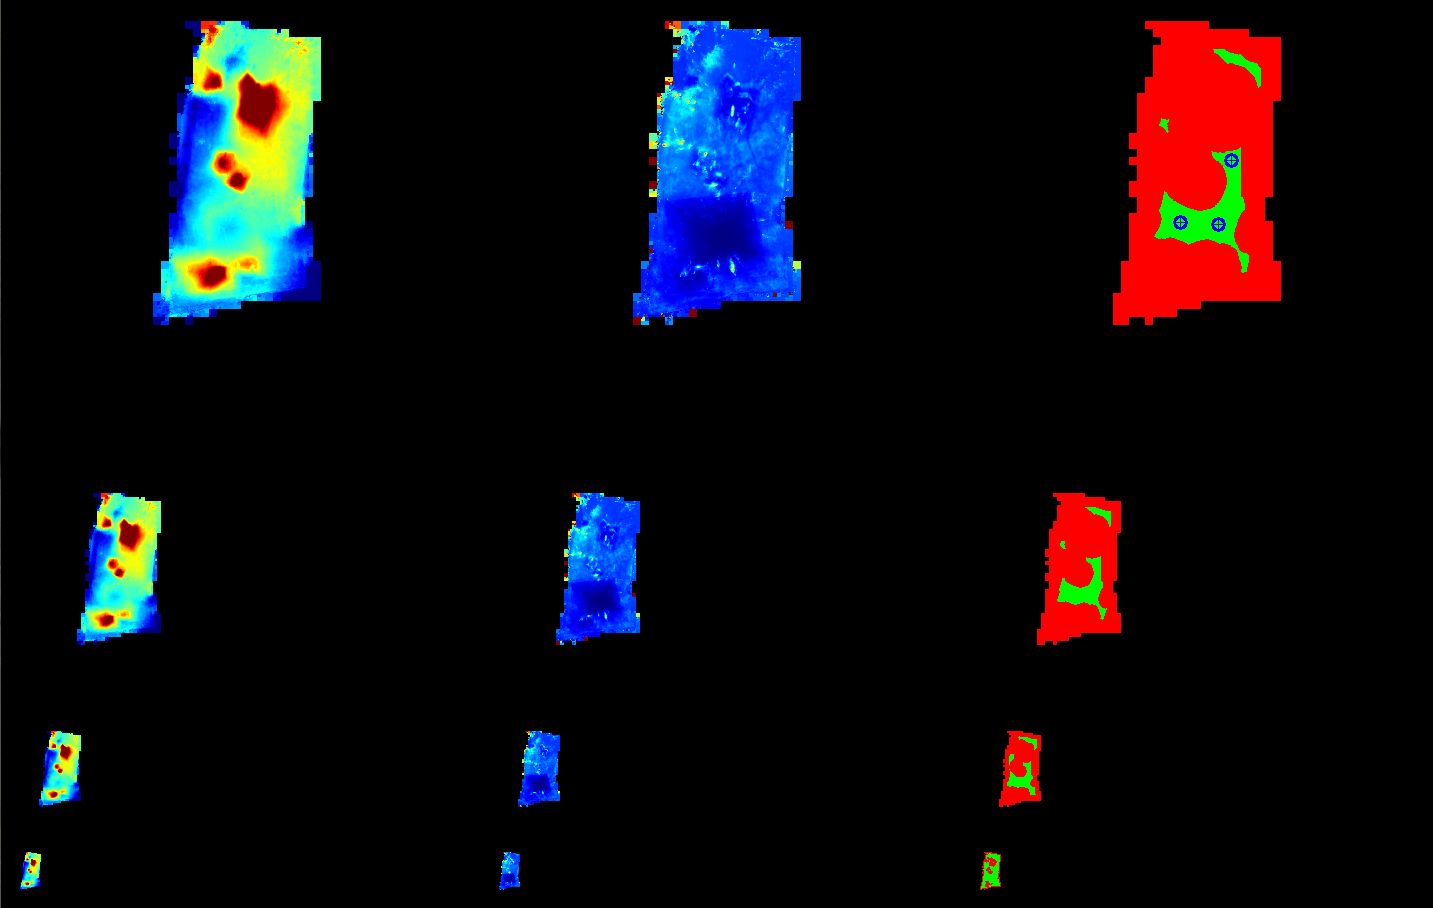
\includegraphics[scale=0.25]{images/stereo_camera_depth/stereo_2.5m.png}
    \caption{Stereo camera depth supplied LSD debug image at 2.5 m altitude}
    \label{qual_stereo_test}
\end{figure}


\begin{figure}[ht!]
    \centering
    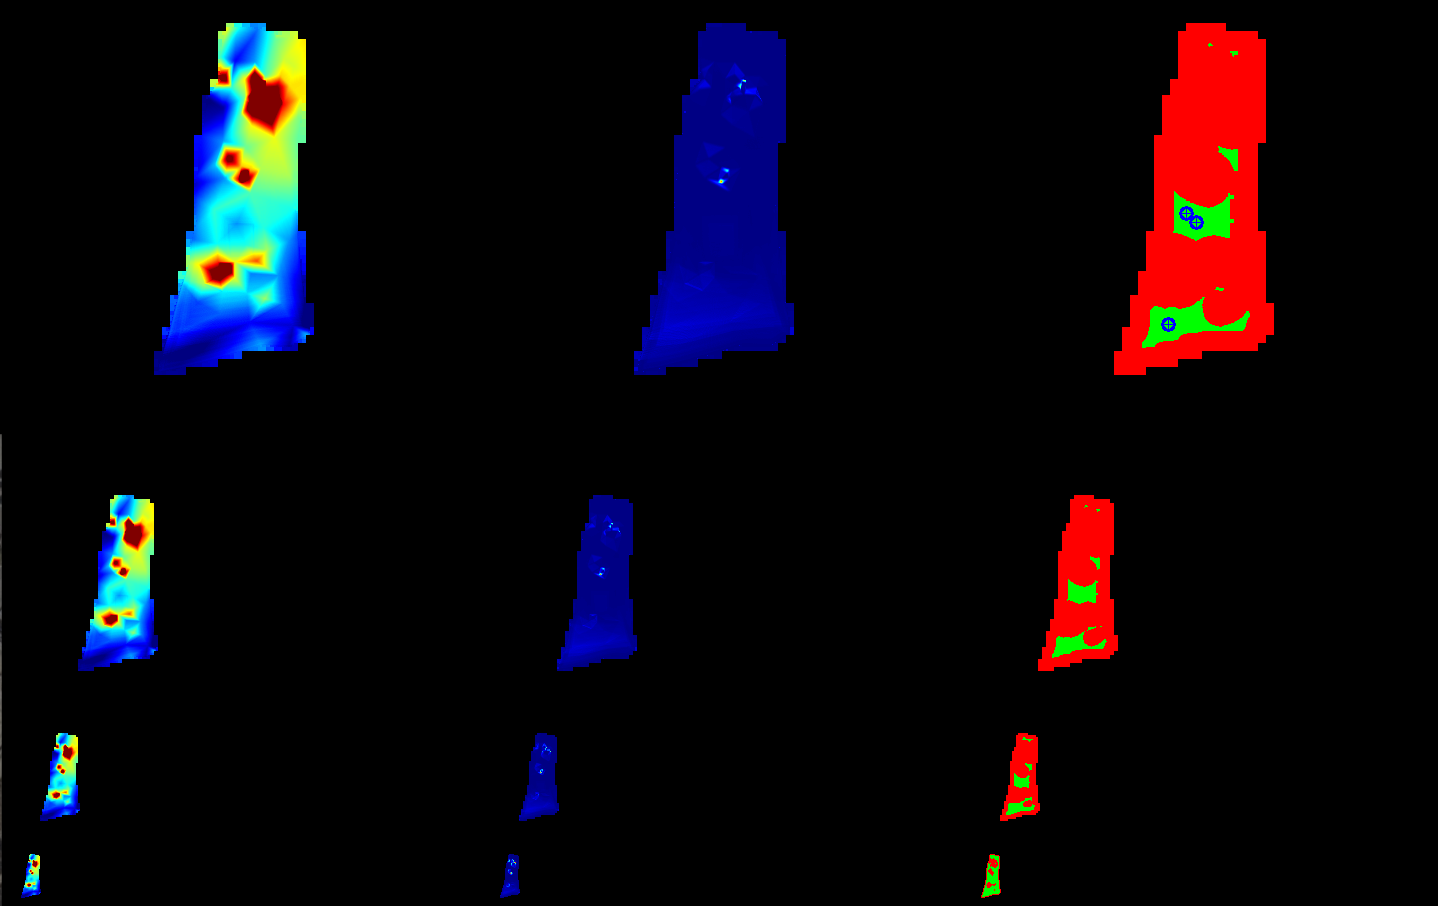
\includegraphics[scale=0.25]{images/stereo_camera_depth/GT_2.5m.png}
    \caption{GT depth supplied LSD debug image at 2.5 m altitude}
    \label{stereo_GT}
\end{figure}

When comparing the result to the ground-truth LSD output, it can be seen that LSD creates a very accurate DEM from the stereo camera depth input. The landing sites detected are reasonable compared to the terrain reference. 

The stereo camera has a relatively small, fixed baseline, so its usage domain is restricted to low altitudes. Therefore, the residual part of a mission is still flown using SFM. 